\documentclass[a4paper,12pt]{article}
%\documentclass[a4paper,10pt]{scrartcl}

\usepackage[margin=0.8in]{geometry}
\usepackage[utf8]{inputenc}
\usepackage{graphicx}

\title{Synchronization of Lines in an Image}
\author{Bnumeros\_Report1}
\date{\today}



\begin{document}
\maketitle

\begin{abstract}
 This report outlines a proposed procedure for synchronising lines of an image that has been corrupted by randomly shifting horizontal lines. The method involves the use of discrete fourier transforms of each line in the given image to determine to what degree each of them was shifted. The end result of the procedure is an image that has been reconstructed to an almost perfect extent, with the edges of the output images being the most notorious unfixed problem.
\end{abstract}

\section{Introduction}

The field of digital image processing aims to modify images through the use of various mathematical operations. This is done by considering images as two dimensional objects and applying signal processing techniques to them in order to manipulate them~\cite{gonzalez1992digital}. This work describes an algorithm written to synchronise an image that has had certain horizontal lines randomly shifted. The algorithm receives as input a corrupted image in file format \texttt{.pgm} (Portable Graymap), which can be read as a two dimensional array. The input image has to have a number of horizontal lines that have been shifted by a random number of pixels, for example fig.~\ref{fig.1}. After passing the input image through the devised algorithm, the output should have most lines shifted into their appropriate location.

\begin{figure}[h!]
\centering
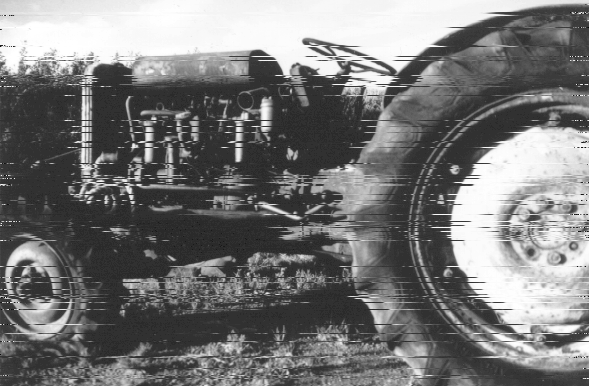
\includegraphics[width=0.75\textwidth]{img/desync2}
\caption{Randomly shifted horizontal lines.}
\label{fig.1}
\end{figure}

The algorithm used to attempt to synchronise the horizontal lines of the given images was written in Python3.5, and imports the libraries \texttt{matplotlib.pyplot} for showing the enhanced image (which is then optionally saved by the user), \texttt{misc} from \texttt{scipy} to read the \texttt{.pgm} input files and write the output file, and \texttt{numpy} since it allows for the use of Discrete Fourier Transform (DFT, which are a fundamental component of the algorithm). Version control was implemented in the development of the algorithm. Consequently, the code is available a public \texttt{github} repository under the following url: \texttt{https://github.com/quietF/NumRep} on the folder \texttt{FT}. There, a short \texttt{README} file details the implementation of the code.

In broad terms, which will be elaborated on later on, the algorithm takes the two dimensional image and compares vertically adjacent lines by calculating the cross correlation between them. From this, the number of pixels that these lines have been shifted is obtained. This allows for a reconstruction of the image. Some limiting cases must be considered to get the enhanced image. It must be said that the developed algorithm can be improved since not all images are perfectly reconstructed. The following sections will elaborate on this. 

\section{Aim and Methods}

The aim of this problem is to take an image in grayscale format with an arbitrary number of horizontally shifted lines and attempt to place them in their right position. Since the line desynchronisation is exclusive to the horizontal direction, i.e. no lines have a vertical shift, it is sensible to divide the two dimensional image into a series of one dimensional objects, where each object is a horizontal line. 

Through the use of various mathematical methods it is possible to find the degree to which each horizontal line has been shifted. The method described, and used, relies on a very strong assumption - vertically adjacent lines can be considered as being approximately equal. The imperfection of the code can be traced back to the assumption not always being true. If two horizontal lines are equal, then their cross correlation would return the degree by which these are shifted. 

This is done by obtaining the Discrete Fourier Transform (DFT) of each horizontal line. Subsequently, the DFT of each line is cross correlated to the DFT of the line directly above. The result of each cross correlation tells whether the line below is shifted relative to the line above.  A comparison with the DFT of the line directly above helps determine whether a shift has occurred.  through the use of Discrete Fourier Transforms of each horizontal line. A comparison between each line and the one directly above it is performed in order to determine by how many pixels the image has been shifted. 


\bibliographystyle{unsrt}
\bibliography{report1}

\end{document}
